\documentclass[10pt,a4paper]{article}
\usepackage[margin=21mm,headheight=15pt]{geometry}
\usepackage[T1]{fontenc}
\usepackage{lmodern,amsmath,amssymb,tikz,graphicx,hyperref,fancyhdr,enumitem}
\usetikzlibrary{arrows.meta,positioning,calc,decorations.pathmorphing}
\definecolor{ink}{RGB}{20,53,78}
\hypersetup{colorlinks=true,urlcolor=ink,linkcolor=ink}
\setlength{\parindent}{0pt}\setlength{\parskip}{5pt}
\emergencystretch=3em
\pagestyle{fancy}\fancyhf{}\fancyfoot[C]{\thepage}
\renewcommand{\headrulewidth}{.3pt}
\newcommand{\task}[2]{\par\medskip{\color{ink}\Large\bfseries #1. #2}\par\smallskip}
\newcommand{\answer}{\par\smallskip\textbf{Worked reasoning.} }
\setlist[enumerate]{label=\textbf{(\alph*)},leftmargin=7mm,itemsep=7pt}
\begin{document}
\fancyhead[L]{\small Control of Dynamical Systems}
\fancyhead[R]{\small Integrated design studies}
{\color{ink}\LARGE\bfseries Integrated design studies}\par
{\large From a physical model to a defensible design decision}\par
\textbf{Exercise sheet -- five integrated problems}\par
{\small\textbf{Evidence boundary.} Original hypothetical scenarios. Derive, calculate and justify decisions; every numerical record is synthetic. Figures are conceptual and not to scale.}
\task{1}{Interacting water tanks: from flow laws to a feasible controller}
Two open tanks have constant areas $A_1=0.02$ m$^2$ and $A_2=0.03$ m$^2$. Their submerged connection obeys
\[
q_{12}=k_{12}\operatorname{sgn}(h_1-h_2)\sqrt{|h_1-h_2|},\qquad
q_2=k_2\sqrt{h_2},
\]
where $k_{12}=0.004$ and $k_2=0.003$ m$^{5/2}$/s. The pump feeds only tank 1. Nominal inflow is $\bar q=0.0012$ m$^3$/s; the measured output is $h_2$. Areas and discharge coefficients are hypothetical. Assume nonnegative levels, no overflow and ideal sensing.
\begin{center}\resizebox{\ifdim\width>.98\linewidth.98\linewidth\else\width\fi}{!}{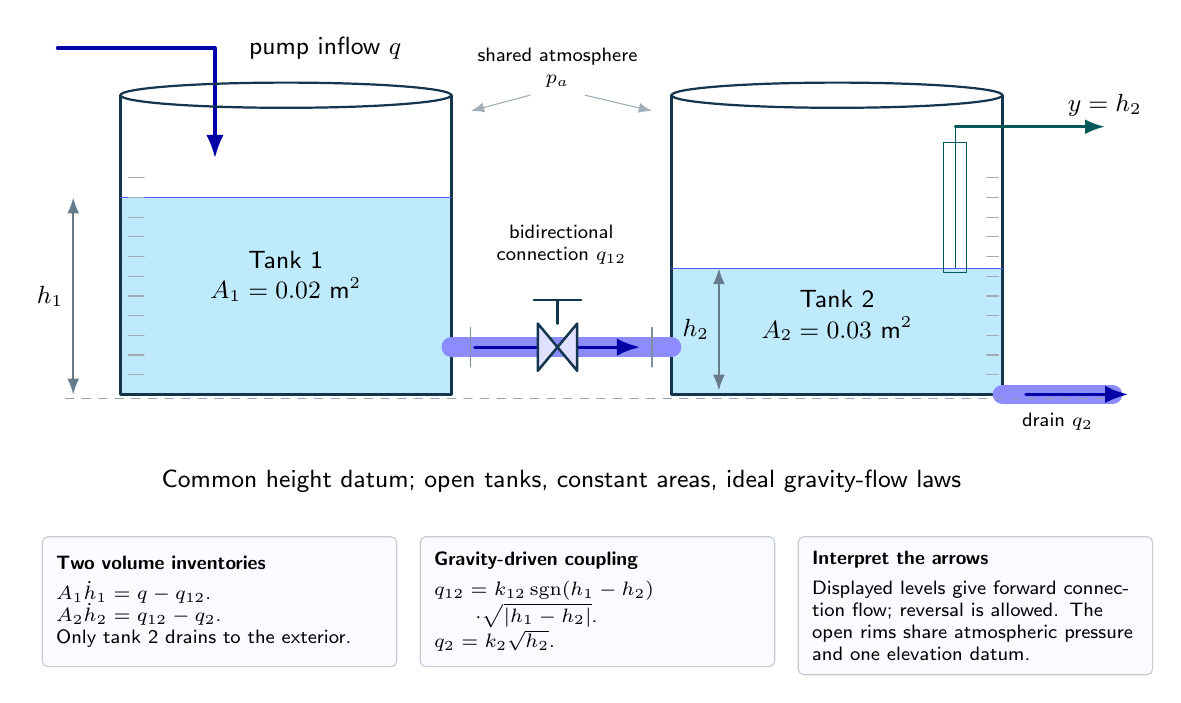
\begin{tikzpicture}[
font=\sffamily\small,>=Latex,line cap=round,line join=round,
wall/.style={draw=ink,line width=1.2pt,fill=blue!5},
water/.style={fill=cyan!25,draw=none},
metal/.style={draw=ink,fill=blue!12,line width=.9pt},
flow/.style={->,draw=blue!65!black,line width=1.2pt},
heat/.style={->,draw=orange!85!black,line width=1.1pt},
measure/.style={->,draw=teal!70!black,line width=.9pt},
dim/.style={<->,draw=ink!65,line width=.6pt},
spring/.style={draw=ink,decorate,decoration={coil,aspect=.5,segment length=4pt,amplitude=3pt}},
wire/.style={draw=ink,line width=1pt},
lab/.style={align=center,font=\sffamily\small},
smalllab/.style={align=center,font=\sffamily\scriptsize}]

\fill[water](1,1)rectangle(5.2,3.5);
\fill[water](8,1)rectangle(12.2,2.6);
\draw[wall,fill=none](1,4.8)--(1,1)--(5.2,1)--(5.2,4.8);
\draw[wall,fill=none](8,4.8)--(8,1)--(12.2,1)--(12.2,4.8);
\draw[blue!65](1,3.5)--(5.2,3.5)(8,2.6)--(12.2,2.6);
\draw[blue!45,line width=7pt](5.2,1.6)--(8,1.6);
\draw[blue!45,line width=7pt](12.2,1)--(13.6,1);
\draw[flow](5.5,1.6)--(7.6,1.6);
\draw[flow](12.5,1)--(13.8,1);
\draw[metal](6.3,1.3)--(6.8,1.9)--(6.8,1.3)--(6.3,1.9)--cycle;
\draw[wire](6.55,1.9)--(6.55,2.2)(6.25,2.2)--(6.85,2.2);
\node[smalllab]at(6.6,2.9){bidirectional\\connection $q_{12}$};
\node[smalllab]at(12.9,.65){drain $q_2$};
\draw[flow](.2,5.4)--(2.2,5.4)--(2.2,4);
\node[lab]at(3.6,5.4){pump inflow $q$};
\node[lab]at(3.1,2.5){Tank 1\\$A_1=0.02$ m$^2$};
\node[lab]at(10.1,2){Tank 2\\$A_2=0.03$ m$^2$};
\draw[dim](.4,1)--node[left]{$h_1$}(.4,3.5);
\draw[dim](8.6,1.05)--node[left]{$h_2$}(8.6,2.6);
\draw[teal!70!black](11.6,2.6)--(11.6,4.4);
\draw[measure](11.6,4.4)--(13.5,4.4)node[above]{$y=h_2$};
\draw[ink!45,dashed](.3,.95)--(13.5,.95);
\node[lab]at(6.6,-.1){Common height datum; open tanks, constant areas, ideal gravity-flow laws};
% REFINED EQUIPMENT DETAILS

% Open tank rims, submerged ports and an instrument associated with h2.
\draw[ink,line width=.8pt](3.1,4.8)ellipse(2.1 and .16);
\draw[ink,line width=.8pt](10.1,4.8)ellipse(2.1 and .16);
\foreach \x in {5.45,7.75}{\draw[ink!55](\x,1.35)--(\x,1.85);}
\draw[teal!70!black](11.45,2.55)rectangle(11.75,4.2);
\foreach \y in {1.25,1.5,...,3.75}{\draw[ink!40](1.1,\y)--(1.3,\y)(12,\y)--(12.15,\y);}
\node[smalllab]at(6.55,5.15){shared atmosphere\\$p_a$};
\draw[ink!40,->](6.2,4.8)--(5.45,4.6);\draw[ink!40,->](6.9,4.8)--(7.75,4.6);

\node[draw=ink!25,fill=blue!2,rounded corners=2pt,anchor=north west,text width=4.15cm,minimum height=1.65cm,inner sep=5pt,align=left,font=\sffamily\scriptsize]at(0.0,-0.8){\textbf{Two volume inventories}\\[3pt]$A_1\dot h_1=q-q_{12}$.\\$A_2\dot h_2=q_{12}-q_2$.\\Only tank 2 drains to the exterior.};
\node[draw=ink!25,fill=blue!2,rounded corners=2pt,anchor=north west,text width=4.15cm,minimum height=1.65cm,inner sep=5pt,align=left,font=\sffamily\scriptsize]at(4.8,-0.8){\textbf{Gravity-driven coupling}\\[3pt]$q_{12}=k_{12}\operatorname{sgn}(h_1-h_2)$\\$\qquad\cdot\sqrt{|h_1-h_2|}$.\\$q_2=k_2\sqrt{h_2}$.};
\node[draw=ink!25,fill=blue!2,rounded corners=2pt,anchor=north west,text width=4.15cm,minimum height=1.65cm,inner sep=5pt,align=left,font=\sffamily\scriptsize]at(9.6,-0.8){\textbf{Interpret the arrows}\\[3pt]Displayed levels give forward connection flow; reversal is allowed. The open rims share atmospheric pressure and one elevation datum.};
\end{tikzpicture}
}\par{\small Interacting tanks share a submerged connection at a common datum. Flow reverses if the level ordering reverses. Only tank 2 drains to the exterior; this is not a cascade with a freely falling inter-tank stream.}\end{center}
\begin{enumerate}
\item Starting from conservation of volume, derive the nonlinear state equations. Find both equilibrium heights and explain why the connection flow depends on a level difference.
\item Linearize about that equilibrium using deviation variables. Derive the transfer function from inflow to the second level, its poles and its DC gain. State where the linearization ceases to be differentiable.
\item Increase the constant inflow by $10^{-4}$ m$^3$/s. Compare the linear and exact equilibrium changes of $h_2$, expressing the error relative to the exact change. Explain why a small input increment is not a universal accuracy certificate.
\item Use deviation PI control $\delta q=k_p(r-\delta h_2)+k_i\int(r-\delta h_2)\,dt$. Derive the characteristic polynomial and the strict stability region for positive gains. Check $k_p=0.001$ m$^2$/s and $k_i=0.0001$ m$^2$/s$^2$.
\item The pump is limited to $0\le q\le0.0015$ m$^3$/s. Can the second level be held at 0.30 m? Determine the highest feasible equilibrium level and describe the implication for integral action.
\item Propose a simulation and identification protocol that could falsify the local model. Include initial conditions, reverse connection flow, numerical convergence and the distinction between simulation and physical validation.
\end{enumerate}

\newpage
\task{2}{Optical isolation with conflicting stiffness and travel requirements}
A hypothetical optical bench of mass $m=8$ kg sits on a parallel spring and viscous damper, with total stiffness $k=3200$ N/m and damping ratio $\zeta=0.08$. The floor displacement is $z(t)$ and payload displacement is $x(t)$, measured about static equilibrium. The floor can oscillate at 40 rad/s with amplitude 0.5 mm. The design brief asks for less payload motion than floor motion, static sag at most 3 mm and relative travel amplitude at most 0.6 mm.
\begin{center}\resizebox{\ifdim\width>.98\linewidth.98\linewidth\else\width\fi}{!}{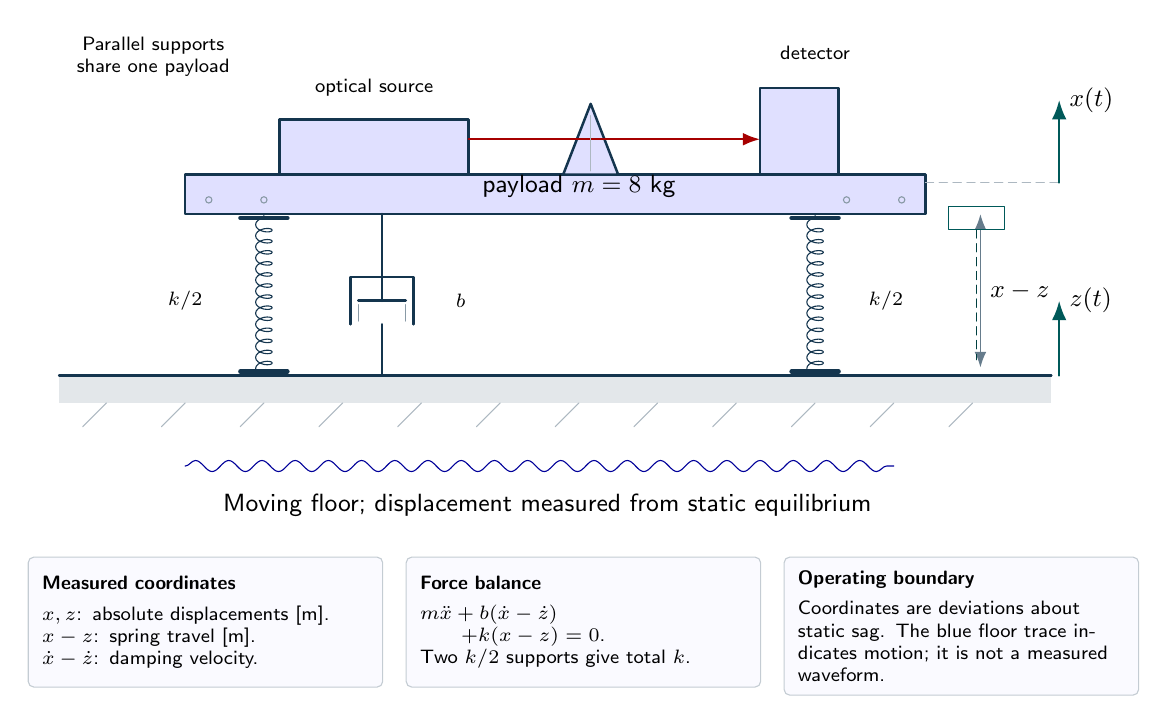
\begin{tikzpicture}[
font=\sffamily\small,>=Latex,line cap=round,line join=round,
wall/.style={draw=ink,line width=1.2pt,fill=blue!5},
water/.style={fill=cyan!25,draw=none},
metal/.style={draw=ink,fill=blue!12,line width=.9pt},
flow/.style={->,draw=blue!65!black,line width=1.2pt},
heat/.style={->,draw=orange!85!black,line width=1.1pt},
measure/.style={->,draw=teal!70!black,line width=.9pt},
dim/.style={<->,draw=ink!65,line width=.6pt},
spring/.style={draw=ink,decorate,decoration={coil,aspect=.5,segment length=4pt,amplitude=3pt}},
wire/.style={draw=ink,line width=1pt},
lab/.style={align=center,font=\sffamily\small},
smalllab/.style={align=center,font=\sffamily\scriptsize}]

\fill[ink!12](.4,.2)rectangle(13,.55);
\draw[ink,line width=1pt](.4,.55)--(13,.55);
\foreach \x in {1,2,...,12}{\draw[ink!35](\x,.2)--++(-.3,-.3);}
\draw[metal](2,2.6)rectangle(11.4,3.1);
\draw[spring](3,.55)--(3,2.6);
\draw[spring](10,.55)--(10,2.6);
\draw[wire](4.5,.55)--(4.5,1.2)(4.1,1.2)--(4.1,1.8)--(4.9,1.8)--(4.9,1.2);
\draw[wire](4.5,2.6)--(4.5,1.5)(4.2,1.5)--(4.8,1.5);
\draw[metal](3.2,3.1)rectangle(5.6,3.8);
\draw[metal](6.8,3.1)--(7.15,4)--(7.5,3.1)--cycle;
\draw[metal](9.3,3.1)rectangle(10.3,4.2);
\draw[red!65!black,->,line width=.7pt](5.6,3.55)--(9.3,3.55);
\node[smalllab]at(4.4,4.2){optical source};
\node[smalllab]at(10,4.65){detector};
\node[lab]at(7,2.95){payload $m=8$ kg};
\node[smalllab]at(2,1.5){$k/2$};\node[smalllab]at(10.9,1.5){$k/2$};
\node[smalllab]at(5.5,1.5){$b$};
\draw[dim](12.1,.65)--node[right]{$x-z$}(12.1,2.6);
\draw[ink!35,densely dashed](11.4,3)--(13.1,3);
\draw[measure](13.1,3)--(13.1,4.05)node[right]{$x(t)$};
\draw[measure](13.1,.55)--(13.1,1.5)node[right]{$z(t)$};
\draw[blue!60!black,decorate,decoration={snake,amplitude=2pt,segment length=12pt}](2,-.6)--(11,-.6);
\node[lab]at(6.6,-1.1){Moving floor; displacement measured from static equilibrium};
% REFINED EQUIPMENT DETAILS

% Fasteners, spring seats and a clearly resolved dashpot piston.
\foreach \x in {2.3,3,10.4,11.1}{\draw[ink!50](\x,2.78)circle(.04);}
\foreach \x in {3,10}{\draw[ink,line width=1.5pt](\x-.3,.6)--(\x+.3,.6)(\x-.3,2.55)--(\x+.3,2.55);}
\draw[ink!50](4.2,1.24)--(4.2,1.45)(4.8,1.24)--(4.8,1.45);
\draw[ink!35](7.15,3.15)--(7.15,3.85);
\draw[teal!70!black](11.7,2.4)rectangle(12.4,2.7);
\draw[teal!50!black,densely dashed](12.05,2.4)--(12.05,.75);
\node[smalllab,anchor=west]at(.5,4.6){Parallel supports\\share one payload};

\node[draw=ink!25,fill=blue!2,rounded corners=2pt,anchor=north west,text width=4.15cm,minimum height=1.65cm,inner sep=5pt,align=left,font=\sffamily\scriptsize]at(0.0,-1.75){\textbf{Measured coordinates}\\[3pt]$x,z$: absolute displacements [m].\\$x-z$: spring travel [m].\\$\dot x-\dot z$: damping velocity.};
\node[draw=ink!25,fill=blue!2,rounded corners=2pt,anchor=north west,text width=4.15cm,minimum height=1.65cm,inner sep=5pt,align=left,font=\sffamily\scriptsize]at(4.8,-1.75){\textbf{Force balance}\\[3pt]$m\ddot x+b(\dot x-\dot z)$\\$\qquad+k(x-z)=0$.\\Two $k/2$ supports give total $k$.};
\node[draw=ink!25,fill=blue!2,rounded corners=2pt,anchor=north west,text width=4.15cm,minimum height=1.65cm,inner sep=5pt,align=left,font=\sffamily\scriptsize]at(9.6,-1.75){\textbf{Operating boundary}\\[3pt]Coordinates are deviations about static sag. The blue floor trace indicates motion; it is not a measured waveform.};
\end{tikzpicture}
}\par{\small An optical payload rests on parallel spring and damping elements. The two springs each have stiffness $k/2$, giving total $k$. Both the floor and payload move; spring extension and damping velocity are relative quantities. Weight is balanced at the static equilibrium about which the model is written.}\end{center}
\begin{enumerate}
\item Draw the force balance and derive both $X/Z$ and $(X-Z)/Z$. Compute the natural frequency and damper coefficient; explain why replacing floor motion by an applied force changes the numerator.
\item Evaluate absolute displacement and relative travel at the stated excitation. Check the two dynamic requirements separately.
\item Show that displacement isolation occurs only above $\sqrt2\,\omega_n$, independently of positive damping. Combine this with the sag requirement to decide whether any passive linear spring can satisfy both specifications at 40 rad/s.
\item Would raising the damping ratio to 0.4 cure the travel issue without a cost? Calculate the two amplitudes at 40 rad/s and compare resonance and high-frequency behavior.
\item Derive an energy balance valid for a moving base. Explain why energy need not decrease even when the damper is passive.
\item Write a justified design decision and a minimum validation plan, including what can and cannot be inferred from a simulated frequency-response curve.
\end{enumerate}

\newpage
\task{3}{A motor speed servo under voltage and load constraints}
A hypothetical DC motor has $R=2\,\Omega$, $L=0.02$ H, $J=0.01$ kg m$^2$, $b=0.02$ N m s/rad, $k_t=0.1$ N m/A and $k_e=0.1$ V s/rad. The load torque is 0.03 N m. The requested speed is 5 rad/s and the voltage limit is $|V|\le2$ V. Positive torque and speed use the same orientation.
\begin{center}\resizebox{\ifdim\width>.98\linewidth.98\linewidth\else\width\fi}{!}{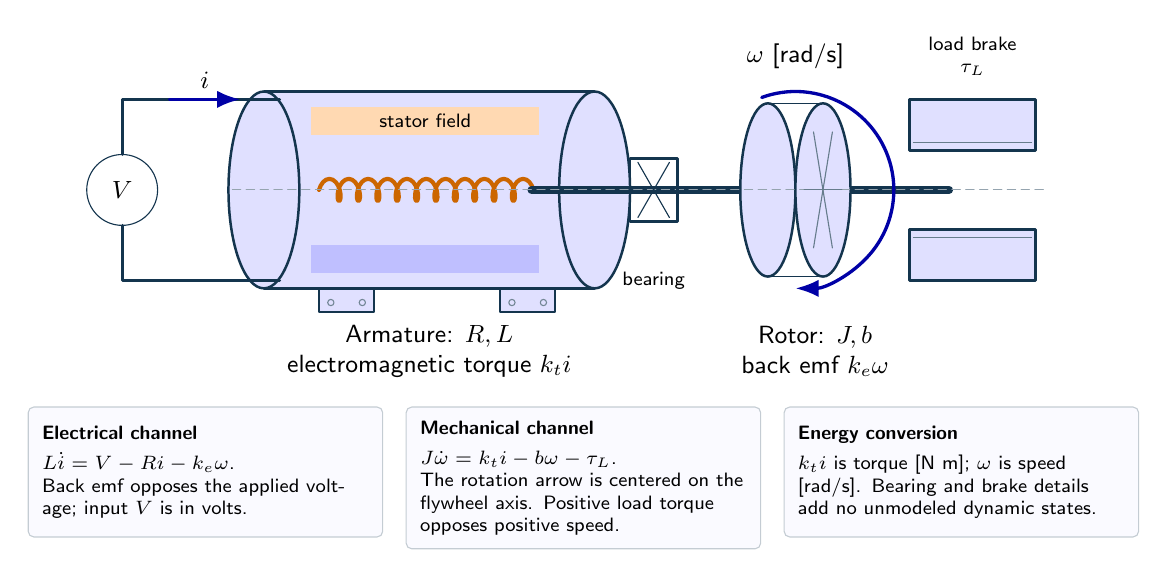
\begin{tikzpicture}[
font=\sffamily\small,>=Latex,line cap=round,line join=round,
wall/.style={draw=ink,line width=1.2pt,fill=blue!5},
water/.style={fill=cyan!25,draw=none},
metal/.style={draw=ink,fill=blue!12,line width=.9pt},
flow/.style={->,draw=blue!65!black,line width=1.2pt},
heat/.style={->,draw=orange!85!black,line width=1.1pt},
measure/.style={->,draw=teal!70!black,line width=.9pt},
dim/.style={<->,draw=ink!65,line width=.6pt},
spring/.style={draw=ink,decorate,decoration={coil,aspect=.5,segment length=4pt,amplitude=3pt}},
wire/.style={draw=ink,line width=1pt},
lab/.style={align=center,font=\sffamily\small},
smalllab/.style={align=center,font=\sffamily\scriptsize}]

\draw[metal](3,1.4)rectangle(7.2,3.9);
\draw[metal](3,2.65)ellipse(.45 and 1.25);
\draw[metal](7.2,2.65)ellipse(.45 and 1.25);
\fill[orange!30](3.6,3.35)rectangle(6.5,3.7);
\fill[blue!25](3.6,1.6)rectangle(6.5,1.95);
\node[smalllab]at(5.05,3.53){stator field};
\draw[orange!80!black,line width=1.5pt,decorate,decoration={coil,segment length=7pt,amplitude=4pt}](3.7,2.65)--(6.5,2.65);
\draw[ink,line width=3pt](6.4,2.65)--(11.7,2.65);
\draw[metal](9.4,2.65)ellipse(.35 and 1.1);
\draw[metal](10.1,2.65)ellipse(.35 and 1.1);
\draw[ink](9.4,3.75)--(10.1,3.75)(9.4,1.55)--(10.1,1.55);
\draw[metal](11.2,1.5)rectangle(12.8,2.15);
\draw[metal](11.2,3.15)rectangle(12.8,3.8);
\node[smalllab]at(12,4.35){load brake\\$\tau_L$};
\draw[flow]($(9.75,2.65)+(110:1.25)$)arc[start angle=110,end angle=-90,radius=1.25];
\node[lab]at(9.75,4.35){$\omega$ [rad/s]};
\draw[wire](3.2,3.8)--(1.2,3.8)--(1.2,3.1)(3.2,1.5)--(1.2,1.5)--(1.2,2.2);
\draw[ink](1.2,2.65)circle(.45);
\node at(1.2,2.65){$V$};
\draw[flow](1.8,3.8)--(2.7,3.8)node[midway,above]{$i$};
\node[lab]at(5.1,.6){Armature: $R,L$\\electromagnetic torque $k_t i$};
\node[lab]at(10,.6){Rotor: $J,b$\\back emf $k_e\omega$};
% REFINED EQUIPMENT DETAILS

% Motor feet, bearing blocks, shaft centerline and flywheel spokes.
\draw[metal](3.7,1.1)rectangle(4.4,1.4);\draw[metal](6,1.1)rectangle(6.7,1.4);
\foreach \x in {3.85,4.25,6.15,6.55}{\draw[ink!60](\x,1.22)circle(.04);}
\draw[ink!45,densely dashed](2.6,2.65)--(12.9,2.65);
\draw[metal,fill=none](7.65,2.25)rectangle(8.25,3.05);
\draw[ink](7.75,2.3)--(8.15,3)(7.75,3)--(8.15,2.3);
\foreach \a in {0,60,...,300}{\draw[ink!65](10.1,2.65)--++({.24*cos(\a)},{.85*sin(\a)});}
\draw[ink!65](11.25,3.25)--(12.75,3.25)(11.25,2.05)--(12.75,2.05);
\node[smalllab]at(7.95,1.5){bearing};

\node[draw=ink!25,fill=blue!2,rounded corners=2pt,anchor=north west,text width=4.15cm,minimum height=1.65cm,inner sep=5pt,align=left,font=\sffamily\scriptsize]at(0.0,-0.1){\textbf{Electrical channel}\\[3pt]$L\dot i=V-Ri-k_e\omega$.\\Back emf opposes the applied voltage; input $V$ is in volts.};
\node[draw=ink!25,fill=blue!2,rounded corners=2pt,anchor=north west,text width=4.15cm,minimum height=1.65cm,inner sep=5pt,align=left,font=\sffamily\scriptsize]at(4.8,-0.1){\textbf{Mechanical channel}\\[3pt]$J\dot\omega=k_ti-b\omega-\tau_L$.\\The rotation arrow is centered on the flywheel axis. Positive load torque opposes positive speed.};
\node[draw=ink!25,fill=blue!2,rounded corners=2pt,anchor=north west,text width=4.15cm,minimum height=1.65cm,inner sep=5pt,align=left,font=\sffamily\scriptsize]at(9.6,-0.1){\textbf{Energy conversion}\\[3pt]$k_ti$ is torque [N m]; $\omega$ is speed [rad/s]. Bearing and brake details add no unmodeled dynamic states.};
\end{tikzpicture}
}\par{\small A voltage-driven motor converts armature current into shaft torque. The rotor and external brake introduce inertia, friction and load torque. The illustrative cutaway does not add magnetic saturation or friction to the stated linear model.}\end{center}
\begin{enumerate}
\item Derive the electrical and mechanical state equations, the voltage-to-speed transfer and the load-to-speed transfer. Identify the approximation made when armature inductance is neglected.
\item Calculate the voltage and current required at the requested speed. Find the largest nonnegative equilibrium speed at the voltage limit and verify steady power balance there.
\item Ignore saturation temporarily and design a PI controller on the reduced plant with desired poles at $-3$ and $-5$ s$^{-1}$. Derive the gains, then test the full electrical-mechanical characteristic polynomial for stability.
\item For a constant feasible reference, explain why ideal PI control removes a constant load offset. Derive the closed-loop load channel and reconcile zero asymptotic error with the infeasible 5 rad/s target.
\item An estimator uses $\widehat{\tau}_L=(k_t/R)V-(b+k_tk_e/R)\omega$. Derive its bias during acceleration and explain what extra information would remove that bias.
\item Propose a revised feasible speed brief and a test that distinguishes controller performance from actuator feasibility. Include anti-windup, initial conditions and parameter uncertainty.
\end{enumerate}

\newpage
\task{4}{Camera tracking: lead-lag design with a network-delay budget}
A normalized camera axis has $G(s)=1/[s(s+1)]$ under unity negative feedback. Design crossover is 3 rad/s and desired phase margin is $55^\circ$. Use $C_{\ell}=K(1+Ts)/(1+\alpha Ts)$, $0<\alpha<1$. A later requirement asks for unit-ramp error at most 0.05. A possible lag stage is $F=(1+s/0.03)/(1+s/0.006)$; a constant delay may also be present.
\begin{center}\resizebox{.88\linewidth}{!}{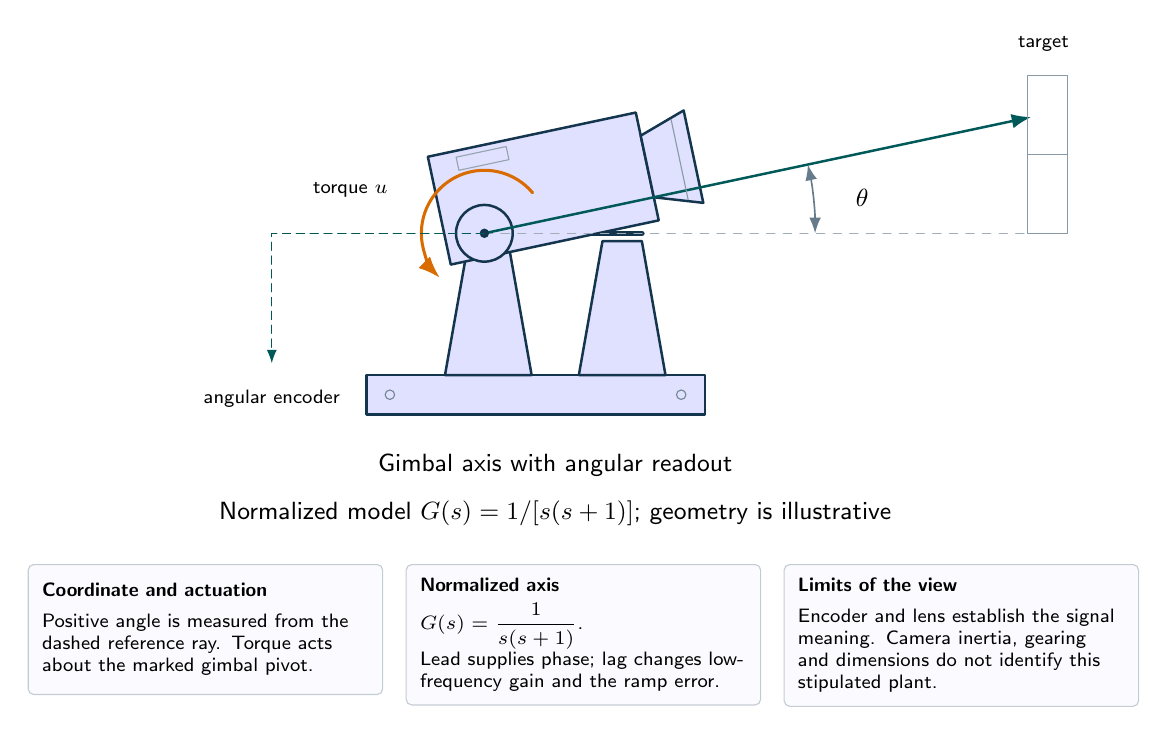
\begin{tikzpicture}[
font=\sffamily\small,>=Latex,line cap=round,line join=round,
wall/.style={draw=ink,line width=1.2pt,fill=blue!5},
water/.style={fill=cyan!25,draw=none},
metal/.style={draw=ink,fill=blue!12,line width=.9pt},
flow/.style={->,draw=blue!65!black,line width=1.2pt},
heat/.style={->,draw=orange!85!black,line width=1.1pt},
measure/.style={->,draw=teal!70!black,line width=.9pt},
dim/.style={<->,draw=ink!65,line width=.6pt},
spring/.style={draw=ink,decorate,decoration={coil,aspect=.5,segment length=4pt,amplitude=3pt}},
wire/.style={draw=ink,line width=1pt},
lab/.style={align=center,font=\sffamily\small},
smalllab/.style={align=center,font=\sffamily\scriptsize}]

\draw[metal](4.3,.4)rectangle(8.6,.9);
\draw[metal](5.3,.9)--(5.6,2.6)--(6.1,2.6)--(6.4,.9)--cycle;
\draw[metal](7,.9)--(7.3,2.6)--(7.8,2.6)--(8.1,.9)--cycle;
\draw[ink,line width=2pt](5.7,2.7)--(7.8,2.7);
\draw[metal,rotate around={12:(5.8,2.7)}](5.3,2.4)rectangle(8,3.8);
\draw[metal,rotate around={12:(5.8,2.7)}](8,2.7)--(8.6,2.5)--(8.6,3.7)--(8,3.5)--cycle;
\draw[metal](5.8,2.7)circle(.36);
\draw[heat]($(5.8,2.7)+(40:.8)$)arc[start angle=40,end angle=225,radius=.8];
\node[smalllab]at(4.1,3.25){torque $u$};
\draw[ink!40,dashed](5.8,2.7)--(12.7,2.7);
\draw[measure](5.8,2.7)--++(12:7.1);
\draw[dim]($(5.8,2.7)+(0:4.2)$)arc[start angle=0,end angle=12,radius=4.2];
\node[lab]at(10.6,3.15){$\theta$};
\draw[ink!50](12.7,2.7)rectangle(13.2,4.7);
\draw[ink!50](12.7,3.7)--(13.2,3.7);
\node[smalllab]at(12.9,5.1){target};
\node[lab]at(6.7,-.25){Gimbal axis with angular readout};
\node[lab]at(6.7,-.85){Normalized model $G(s)=1/[s(s+1)]$; geometry is illustrative};
% REFINED EQUIPMENT DETAILS

% Resolved camera lens, mounting bolts, encoder readout and pivot.
\foreach \x in {4.6,8.3}{\draw[ink!60](\x,.65)circle(.06);}
\draw[ink!50,rotate around={12:(5.8,2.7)}](8.42,2.58)--(8.42,3.62);
\draw[ink!45,rotate around={12:(5.8,2.7)}](5.65,3.55)rectangle(6.3,3.72);
\fill[ink](5.8,2.7)circle(.06);
\draw[teal!70!black,densely dashed,->](5.8,2.7)--(3.1,2.7)--(3.1,1.05);
\node[smalllab]at(3.1,.6){angular encoder};

\node[draw=ink!25,fill=blue!2,rounded corners=2pt,anchor=north west,text width=4.15cm,minimum height=1.65cm,inner sep=5pt,align=left,font=\sffamily\scriptsize]at(0.0,-1.5){\textbf{Coordinate and actuation}\\[3pt]Positive angle is measured from the dashed reference ray. Torque acts about the marked gimbal pivot.};
\node[draw=ink!25,fill=blue!2,rounded corners=2pt,anchor=north west,text width=4.15cm,minimum height=1.65cm,inner sep=5pt,align=left,font=\sffamily\scriptsize]at(4.8,-1.5){\textbf{Normalized axis}\\[3pt]$G(s)=\dfrac{1}{s(s+1)}$.\\Lead supplies phase; lag changes low-frequency gain and the ramp error.};
\node[draw=ink!25,fill=blue!2,rounded corners=2pt,anchor=north west,text width=4.15cm,minimum height=1.65cm,inner sep=5pt,align=left,font=\sffamily\scriptsize]at(9.6,-1.5){\textbf{Limits of the view}\\[3pt]Encoder and lens establish the signal meaning. Camera inertia, gearing and dimensions do not identify this stipulated plant.};
\end{tikzpicture}
}\par{\small The same camera axis is used in laboratory 08; laboratory 07 supplies the communication-delay interpretation.}\end{center}
\begin{enumerate}
\item Show why scalar gain alone cannot meet the crossover and phase-margin targets simultaneously. Determine the needed lead phase.
\item Place maximum lead at the design crossover and derive $\alpha,T,K$. Verify both the magnitude and phase conditions rather than using rounded parameters alone.
\item Find the lead-only ramp error. Add the specified lag, normalize its magnitude at 3 rad/s by a scalar $g$, and compute the new ramp error and phase margin. Does the combined design satisfy both original requirements?
\item For the combined compensator, derive the first constant-delay stability boundary and the maximum delay that retains $40^\circ$ phase margin. Assess 0.09 s delay.
\item Derive the high-frequency measurement-noise-to-control limit. Explain why small output noise need not imply small actuator activity.
\item Write a defensible acceptance decision for the current design and specify which calculations must be repeated after retuning.
\end{enumerate}

\newpage
\task{5}{Two-zone temperature regulation with estimation and sampled actuation}
Two lumped thermal zones each have capacity 10 J/K. Their mutual conductance is 0.5 W/K; conductances to a fixed ambient are 1 and 0.5 W/K, respectively. Heat input acts in zone 1 and only zone 2 is measured. States are temperature deviations in K. The nominal feedback pole targets are $-0.20,-0.35$ s$^{-1}$; observer targets are $-0.8,-1.0$ s$^{-1}$. A later implementation holds each input constant between samples.
\begin{center}\resizebox{.88\linewidth}{!}{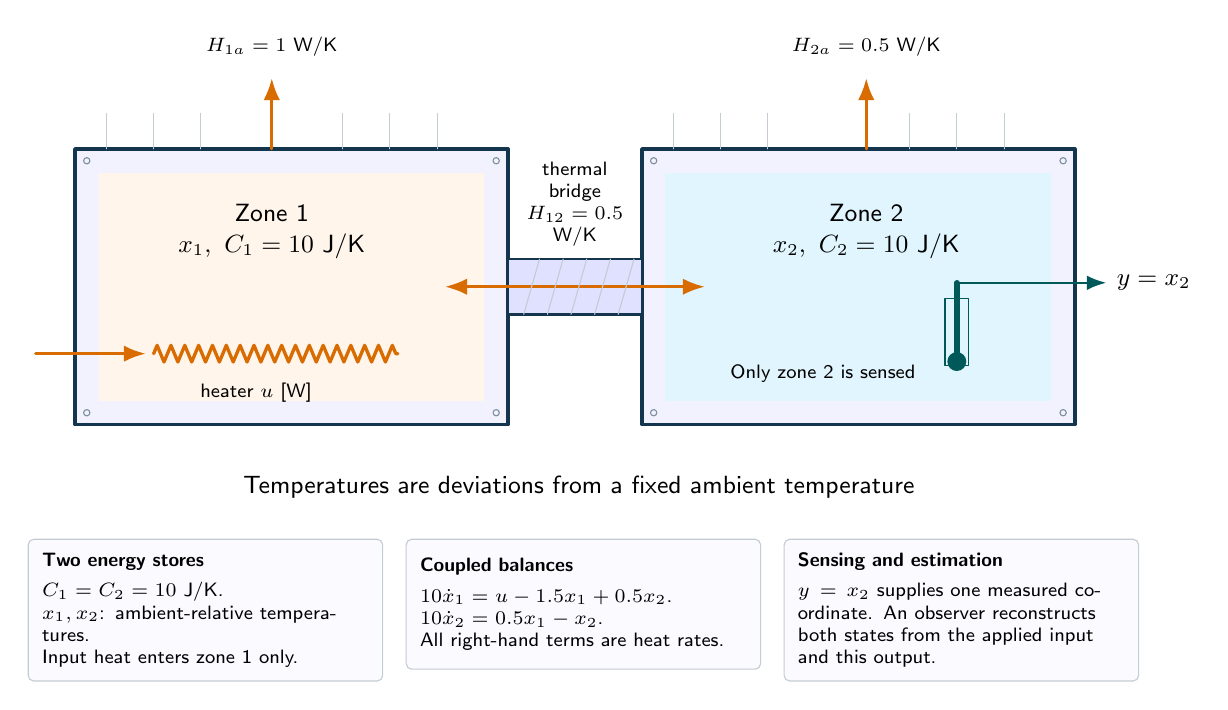
\begin{tikzpicture}[
font=\sffamily\small,>=Latex,line cap=round,line join=round,
wall/.style={draw=ink,line width=1.2pt,fill=blue!5},
water/.style={fill=cyan!25,draw=none},
metal/.style={draw=ink,fill=blue!12,line width=.9pt},
flow/.style={->,draw=blue!65!black,line width=1.2pt},
heat/.style={->,draw=orange!85!black,line width=1.1pt},
measure/.style={->,draw=teal!70!black,line width=.9pt},
dim/.style={<->,draw=ink!65,line width=.6pt},
spring/.style={draw=ink,decorate,decoration={coil,aspect=.5,segment length=4pt,amplitude=3pt}},
wire/.style={draw=ink,line width=1pt},
lab/.style={align=center,font=\sffamily\small},
smalllab/.style={align=center,font=\sffamily\scriptsize}]

\draw[wall](.6,.7)rectangle(6.1,4.2);
\draw[wall](7.8,.7)rectangle(13.3,4.2);
\fill[orange!8](.9,1)rectangle(5.8,3.9);
\fill[cyan!12](8.1,1)rectangle(13,3.9);
\draw[metal](6.1,2.1)rectangle(7.8,2.8);
\draw[heat,<->](5.3,2.45)--(8.6,2.45);
\node[smalllab]at(6.95,3.5){thermal\\bridge\\$H_{12}=0.5$\\W/K};
\draw[orange!85!black,line width=1.2pt,decorate,decoration={zigzag,segment length=5pt,amplitude=3pt}](1.6,1.6)--(4.7,1.6);
\draw[heat](.1,1.6)--(1.5,1.6);
\node[smalllab]at(2.9,1.1){heater $u$ [W]};
\node[lab]at(3.1,3.15){Zone 1\\$x_1,\ C_1=10$ J/K};
\node[lab]at(10.65,3.15){Zone 2\\$x_2,\ C_2=10$ J/K};
\draw[teal!70!black,line width=2pt](11.8,1.5)--(11.8,2.5);
\fill[teal!70!black](11.8,1.5)circle(.12);
\draw[measure](11.8,2.5)--(13.7,2.5)node[right]{$y=x_2$};
\draw[heat](3.1,4.2)--(3.1,5.1);
\draw[heat](10.65,4.2)--(10.65,5.1);
\node[smalllab]at(3.1,5.5){$H_{1a}=1$ W/K};
\node[smalllab]at(10.65,5.5){$H_{2a}=0.5$ W/K};
\node[lab]at(7,-.1){Temperatures are deviations from a fixed ambient temperature};
% REFINED EQUIPMENT DETAILS

% Distinct thermal masses and finite conductive contact.
\foreach \x in {1,1.6,2.2,4,4.6,5.2}{\draw[ink!25](\x,4.2)--(\x,4.65);}
\foreach \x in {8.2,8.8,9.4,11.2,11.8,12.4}{\draw[ink!25](\x,4.2)--(\x,4.65);}
\foreach \x in {6.3,6.6,6.9,7.2,7.5}{\draw[ink!25](\x,2.1)--(\x+.2,2.8);}
\foreach \x/\y in {.75/.85,.75/4.05,5.95/.85,5.95/4.05,7.95/.85,7.95/4.05,13.15/.85,13.15/4.05}{\draw[ink!55](\x,\y)circle(.04);}
\draw[teal!70!black](11.65,1.45)rectangle(11.95,2.3);
\node[smalllab]at(10.1,1.35){Only zone 2 is sensed};

\node[draw=ink!25,fill=blue!2,rounded corners=2pt,anchor=north west,text width=4.15cm,minimum height=1.65cm,inner sep=5pt,align=left,font=\sffamily\scriptsize]at(0.0,-0.75){\textbf{Two energy stores}\\[3pt]$C_1=C_2=10$ J/K.\\$x_1,x_2$: ambient-relative temperatures.\\Input heat enters zone 1 only.};
\node[draw=ink!25,fill=blue!2,rounded corners=2pt,anchor=north west,text width=4.15cm,minimum height=1.65cm,inner sep=5pt,align=left,font=\sffamily\scriptsize]at(4.8,-0.75){\textbf{Coupled balances}\\[3pt]$10\dot x_1=u-1.5x_1+0.5x_2$.\\$10\dot x_2=0.5x_1-x_2$.\\All right-hand terms are heat rates.};
\node[draw=ink!25,fill=blue!2,rounded corners=2pt,anchor=north west,text width=4.15cm,minimum height=1.65cm,inner sep=5pt,align=left,font=\sffamily\scriptsize]at(9.6,-0.75){\textbf{Sensing and estimation}\\[3pt]$y=x_2$ supplies one measured coordinate. An observer reconstructs both states from the applied input and this output.};
\end{tikzpicture}
}\par{\small The same two-zone plant is used in laboratory 10. Laboratory 11 supplies the sampling and held-input interpretation; its RC plant is not substituted here.}\end{center}
\begin{enumerate}
\item Derive $A,B,C$ from heat balances and test controllability and observability. Explain physically what is lost when the mutual conductance is zero.
\item Find $K$ for $u=-Kx+Nr$ and the reference prefilter $N$. Derive the equilibrium heat input and distinguish transient and equilibrium feasibility for a 0.5 K step with a 2 W upper limit.
\item Find the observer gain and derive the augmented dynamics in coordinates $[x,e]$, where $e=x-\hat x$. Explain which control signal the observer must receive under saturation.
\item An unknown constant heat disturbance enters zone 2. Explain why the prefilter does not remove its offset and test whether adding an error integrator preserves controllability.
\item For full-state sampled feedback with the same $K$, derive the exact held-input transition matrix. Compare sampling periods 1 s and 10 s. Explain why exponentiating $A-BK$ would answer a different implementation question.
\item Specify a validation protocol that separates observer convergence, constant bias, sampled stability and experimental evidence.
\end{enumerate}

\end{document}
